\begin{block}{Study Area \& Variable Definitions}
    \begin{figure}
        \centering
        \caption{Composite anomalies of \SI{500}{\hecto\pascal} geopotential height (color) and precipitable water (contours) from 4 days preceding regional intense precipitation days in the Ohio River Basin to one day following.}
        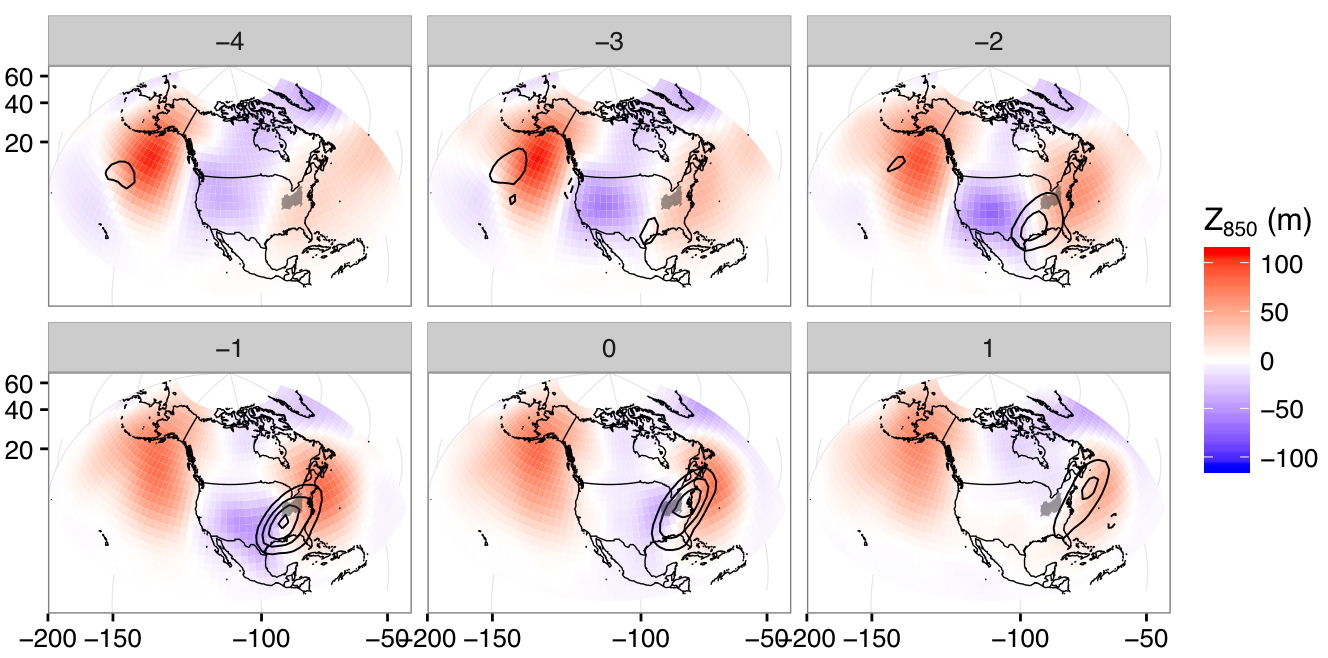
\includegraphics[width=\columnwidth]{../FigExternal/djf_composites}
        \label{fig:djf-composites}
    \end{figure}
    Study of regional intense precipitation events in the Ohio River Basin (\cref{fig:djf-composites}) reveals the dominance of a ridge (somtimes stationary, sometimes transient) over the Western Atlantic and a transient cyclone propagating eastward.
    To study this, we define the following variables, separated into planetary-scale and synoptic-scale:
    \begin{description}
        \item[Moisture] the daily net moisture flux into Ohio River Basin region (\cref{fig:study-area}, green box)
        \item[Planetary] 30-day moving average of the PNA and NAO indices from the CPC
        \item[Synoptic] Mean SST anomaly over the Gulf of Mexico (\cref{fig:study-area}, blue); and the \SI{850}{\hecto\pascal} the geopotential height anomalies over the West Atlantic (\cref{fig:study-area}, purple) and the Eastern United States (red).
    \end{description}
    \begin{figure}
        \centering
        \includegraphics[width=0.8\columnwidth]{map_inset}
        \caption{Study Area. Shaded area shows the Ohio River Basin.}
        \label{fig:study-area}
    \end{figure}
\end{block}
